\subsection{Build software}
  Before discussing the build stage, it's important to understand the multiple environments used in development.

  \begin{figure}[H]
    \centering
    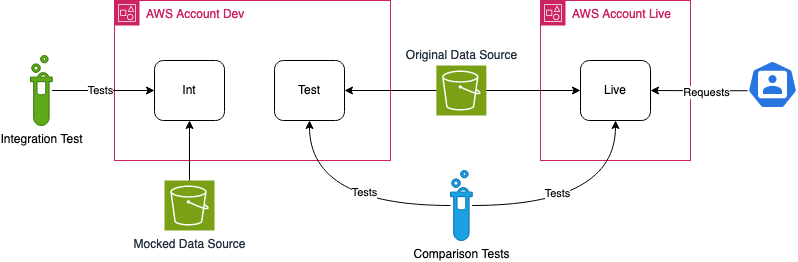
\includegraphics[width=8cm]{assets/environments.drawio.png}
    \caption{Diagram showing the different environments used by SpaceChimp.}
    \label{fig:environments}
  \end{figure}

  The above figure illustrates where the pipelines get their data from dependant on the environment, as well as what tests access said environment.
  We have 3 environments, int, test and live, with test mimicking live (Wiggins, 2017). This allows us to use the test environment to protect live from 
  any bugs or errors introduced by a task whilst also allowing the testing of outputs between old and software (Zheng, 2021). However when running on test
  and live we don't have control over the data source and the events it sends out to the pipeline, thus making it hard to test certain scenarios and features.
  This is where the int environment is used, we mock the data source used on test/live but have full control over what is added and removed, This allows 
  us to routinely check all edge cases and features are working as expected.

  \vspace{0.2cm}

  The build stage consists of writing and testing the software and resembles the flow of our kanban board.

  \begin{figure}[H]
    \centering
    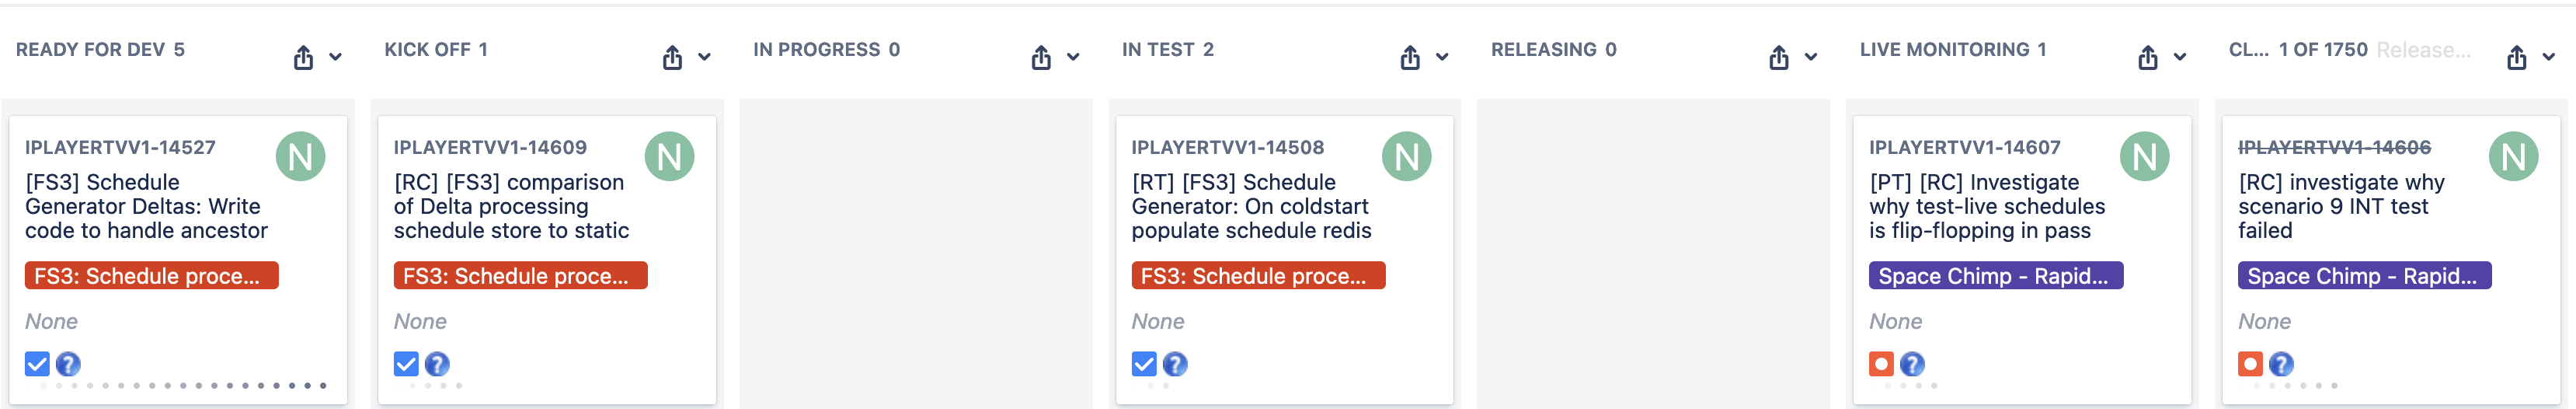
\includegraphics[width=10cm]{assets/kanbanBoard.png}
    \caption{SpaceChimps kanban board.}
    \label{fig:kanbanBoard2}
  \end{figure}

  \begin{itemize}
    \item \textbf{Ready for dev} - Tasks that are ready to be picked up for development.
    \item \textbf{Kick-off} - Tasks that need a test kick-off, which is not the same as the previous sections kick-off. This is where developers
    discuss the task with a member of the test team and determine the Acceptance Criteria (ACs) and test approach for the task.
    \item \textbf{In Progress} - Tasks that are being developed and worked on.
    \item \textbf{In Test} - Task has been completed and changes are on the test environment. A member of the test team can now test the ticket
    based on the previous discussions had in the kick-off. If things have changed during development, an additional hand-over with the test team 
    is done to discuss the new changes.
    \item \textbf{Releasing} - After a ticket task has been tested and has met the specified ACs, the task is moved to the releasing column signifying 
    that is ready to be deployed to the live environment.
    \item \textbf{Live monitoring} - Tasks in this column need to be monitored on the live environment to make sure that the change is functioning as expected.
  \end{itemize}

  \begin{figure}[H]
    \centering
    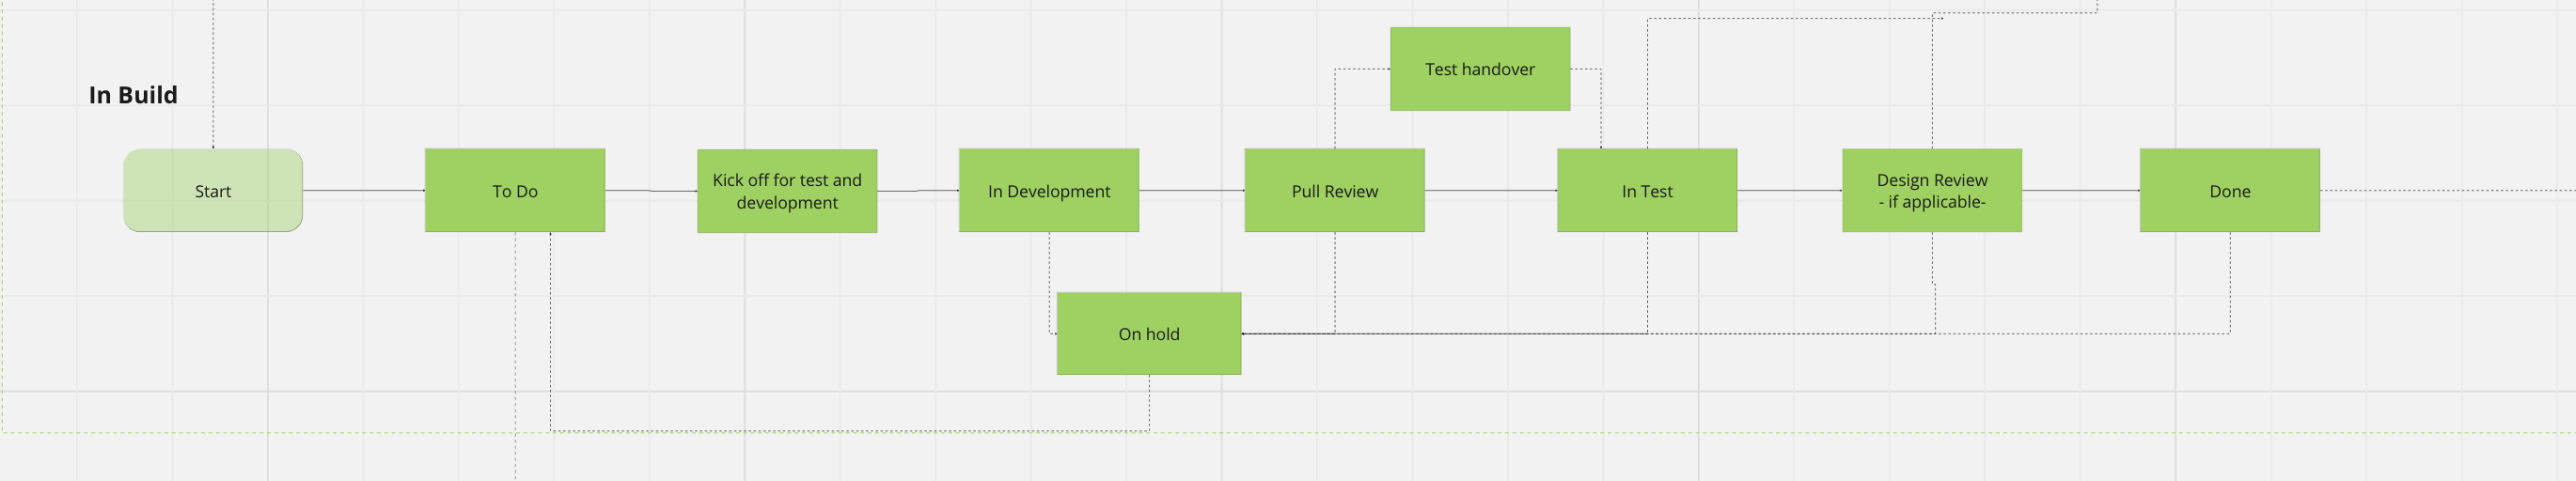
\includegraphics[width=8cm]{assets/workflow/build.png}
    \caption{Build stage of our of working.}
    \label{fig:workflowBuild}
  \end{figure}

  I will now discuss the 4 key components/features that were built during this stage, along with decisions and challenges that occurred during development.

  \newpage
  \subsubsection{Delta/change lambda}
  Before notification events were being processed, schedules relied on the coldstarting/refreshing of data every 15 minutes. The delta lambda is the 
  the component that moves away from this paradigm and is the main component in this project. I have separated this section into the different types
  of notifications the component can receive, schedule updates and deletes and catalogue updates and deletes. But before delving into that, a bit of extra
  information is required about the build.

  \vspace{0.2cm}
  In the old system there was no link between episodes and schedules. We now need one, as an certain changes to episodes can change what a schedule 
  contains. For this reason it was decided that a new field could be added to episode, the broadcast\_list field. This would contain a list of all 
  schedules that an episode was referenced in.

  In addition to this, an architectural decision was made, before me taking on the project for this report, to have all schedule documents be in one keyspace,
  this can be seen in \hyperref[sec:AppendixF]{\textbf{Appendix F}}. 
  This making it easy to return all the relevant data on partner requests from our API and now with an additional field, making it so catalogue schemas would 
  not have to be changed. To do this all data relating to any current schedules offered must be copied over from the catalogue redis keyspace to the schedule
  redis keyspace, with the broadcast\_list field being added only to the schedules version of the object. The below figure shows how this works on a
  schedule update.

  \begin{figure}[H]
    \centering
    \includegraphics[width=12cm]{diagrams/activity/Populate Catalogue Items.png}
    \caption{Activity diagram showing logic of populating schedule redis.}
    \label{fig:scheduleRedisPopulationActivity}
  \end{figure}

  There's 3 options that can happen here:
  \begin{enumerate}
    \item If the episode is already in the schedules store, then we need to add a link to the current schedule being updated if it doesn't
    already reference it. 
    \item If it's not in the schedules store, but is in the catalogue store, then it needs to be copied over and have the current schedule
    being updated referenced in it's broadcast list.
    \item If it's not in either store, then a stub must be made, this stub has a unique identifier (pid), a type of \emph{episode\_stub} and 
    a broadcast list, that in this case holds the schedule currently being updated.
  \end{enumerate}

  The episode stub is required, despite it containing no useful information to the schedules tilting and other fields and is also discarded when a
  partner requests said schedule. It is required because of the event driven nature of the new system and the broadcast list it contains. With a stub in 
  the store, when an episode update is processed for that stub it can now also update all the schedules associated with it, immediately populating tilting
  and descriptions for all.

  As will be discussed in the following sections, different types of notifications can affect different kinds of data. Below is a table showing the 
  relations between types of updates and what can be affected. The garbage collector will be discussed later in the report, but is also included in 
  the table for completeness.

  \begin{table}[H]
    \centering
    \begin{tabular}{|p{0.3\textwidth}|p{0.15\textwidth}|p{0.15\textwidth}|p{0.15\textwidth}|}
      \hline
      & Schedule & Episode & Ancestor \\ \hline
      Schedule Update & \ding{51} & \ding{51} \ding{55} & \ding{51} \\ \hline
      Schedule Delete & \ding{55} & \ding{55} & \\ \hline
      Episode Update & \ding{51} & \ding{51} & \ding{51} \\ \hline
      Ancestor Update & \ding{51} &  & \ding{51} \\ \hline
      Garbage Collector &  &  & \ding{55} \\ \hline
    \end{tabular}
    \caption{Table showing how different types of notification can affect stored data (\ding{51} updates, \ding{55} deletes).}
  \end{table}


  \paragraph{Schedule Updates}
  Schedule updates refer to either the updating of a schedule, or the creation of a new schedule. There are some guards around whether the 
  schedule exists, then all catalogue data associated with the schedule is copied from the catalogue store to the schedule store, if it's is 
  not already there. This data can then be used to transform everything into the final schedule, where if any valid changes have been made, the 
  new schedule is stored.

  \begin{figure}[H]
    \centering
    \includegraphics[width=8cm]{diagrams/activity/Schedule Update.png}
    \caption{Activity diagram showing logic when schedule update notification received.}
    \label{fig:scheduleUpdateActivity}
  \end{figure}

  There is an edge case specified in the above diagram, where a broadcast within a schedule changes the episode that it's going to play. 
  In this case we have to either tidy up the old episodes broadcast list to no longer contain a reference to the schedule, or, if that episode no 
  longer references any schedules, remove it from the schedule store.

  \begin{figure}[H]
    \centering
    \includegraphics[width=8cm]{diagrams/activity/Broadcast Changed.png}
    \caption{Activity diagram showing logic to handle broadcast episode change.}
    \label{fig:broadCastChangeActivity}
  \end{figure}

  \paragraph{Schedule Deletes}
  Schedule deletes are one of the simpler events. Other than some basic guards to check objects exists in redis, all episode object referenced in 
  the schedules broadcasts have the schedule being deleted removed from their broadcast list. If this list is empty then that episode is also removed
  from the schedule store. After all this is done, the schedule is also removed from the schedule store.

  \begin{figure}[H]
    \centering
    \includegraphics[width=8cm]{diagrams/activity/Schedule Delete.png}
    \caption{Activity diagram showing logic when schedule delete notification received.}
    \label{fig:scheduleDeleteActivity}
  \end{figure}

  \paragraph{Catalgoue Updates}
  Catalogue updates must also be processed by the schedule generator as they contain information about titling, programme descriptions and more.


  \begin{figure}[H]
    \centering
    \includegraphics[width=6cm]{diagrams/activity/Episode Update.png}
    \includegraphics[width=6cm]{diagrams/activity/Ancestor Update.png}
    \caption{Activity diagrams showing logic when episode (left) and ancestor update (right) notifications received.}
    \label{fig:scheduleUpdateCatalogueActivity}
  \end{figure}

  Episode and ancestor updates are similar. Episode updates must update themselves but also that episodes parents as
  the parents contain additional tilting information required for the schedule to be accurate.

  Due to this titling information being held at multiple levels of the catalogue data, when an ancestor is updated it must update itself,
  but then also find all episodes in the schedule store that are dependant on it.

  Episodes contain a list of schedules that reference it. These schedules must be updated, so a method was created that could handle these
  schedule changes in a batch form.

  \begin{figure}[H]
    \centering
    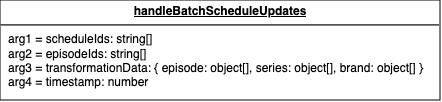
\includegraphics[width=8cm]{assets/handleBatchScheduleInterface.drawio.png}
    \caption{Class diagram showing the interface for the handling schedule updates triggered by catalogue notifications.}
    \label{fig:catalogueTriggeredScheduleUpdateClass}
  \end{figure}

  The method used the above interface and could be called the same way when updating an episode or an ancestor. The data includes:
  \begin{itemize}
    \item \textbf{scheduleIds} - Schedules in episodes broadcast lists.
    \item \textbf{episodeIds} - Episodes effected by the change, singular on episode update, multiple on ancestor update.
    \item \textbf{transformationData} - Episode/series/brand data needed to transform the all schedules.
    \item \textbf{timestamp} - Used for consistent update time on all updates.
  \end{itemize}

  Using this interface logic can then carried out to only update the broadcasts that have changed within a schedule instead of the 
  entire schedule itself.

  \begin{figure}[H]
    \centering
    \includegraphics[width=6cm]{diagrams/activity/Catalogue update triggered schedule updates.png}
    \caption{Activity diagram showing logic that happens when a catalogue notification triggers schedule updates.}
    \label{fig:catalogueTriggeredScheduleUpdateActivity}
  \end{figure}

  \paragraph{Catalogue Deletes}
  It was determined during the spike that catalogue deletes would not need to be processed due to the creation of the garbage collector removing 
  orphaned ancestor items, and schedule events taking care of episode removals. This saves a lot of additional lambda invokes over time.

  \newpage
  \subsubsection{Coldstarts}
  We use the term coldstart to refer to the refreshing of all data, in schedules terms all schedules will be checked to see if an update has occurred.
  This is not related to a cold start/boot in relation to serverless architectures (Microsoft Azure, 2018), although this is something that can affect 
  our lambdas. We already had a coldstart in place but changes would have to be made to work with the new delta/notifications environment.

  \begin{figure}[H]
    \centering
    \includegraphics[width=8cm]{diagrams/activity/Intial Coldstart Design.png}
    \caption{Activity diagram showing initial idea for coldstart changes.}
    \label{fig:initialColdstart}
  \end{figure}

  The above diagram shows the initial design for how the coldstart would function. The changes seem relatively simple:
  \begin{enumerate}
    \item Disable triggering of lambda on delta notification event. This is so no changes can interfere with the refresh of data.
    \item Purge the queue of updates before starting processing to stop unnecessary triggers of the lambda after the cold start has finished.
    \item Populate the redis with all the catalogue data it needs, this is done on schedule updates also. 
    \item Re-enable the triggering of lambda on delta notification event.
  \end{enumerate}

  Disabling and enabling of the lambda trigger can be achieved through the UpdateEventSourceMapping api (Amazon Web Services, 2024l) provided by AWS. 
  At the start, the trigger can be disabled, then re-enabled once the coldstart is finished.

  \begin{figure}[H]
    \centering
    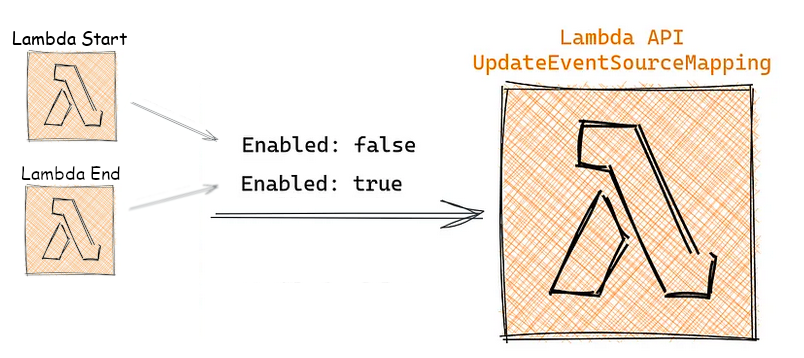
\includegraphics[width=8cm]{assets/lambdaMapping.png}
    \caption{Diagram edited from Charles (2021) to show lambda mapping states.}
    \label{fig:lambdaMapping}
  \end{figure}

  Purging the SQS queue of delta notifications can also be done though a similar API and the population of redis is already done per schedule, so 
  this seems like an easy switchover to work in the new world of delta notifications.

  However, as work began the code grew more and more complex, due mainly to the new logic of copying data over into the new schedule redis keyspace.
  Maintaining the broadcast list in the episodes would mean making the population logic complex and hard to follow. Code complexity can be a huge 
  problem with developers not wanting to edit the code in fear of breaking the current workings, difficulty to maintain 
  (Mateus, Andre, 2022 and Olbrich et al, 2009) and the \textit{truck/bus factor} which illustrates how hard it would be for a new team member to 
  understand with no help from the creator (Avelino et al, 2016). In addition to this, a study done by (Taibi et al, 2017) found that 
  \textit{'Smells related to size and complexity are considered harmful by a higher percentage of participants than others.'}. The system created is 
  complex and has multiple inputs that can interfere with each other, the same study also found that this higher complexity is less likely to be 
  refactored in the future (Taibi et al, 2017).

\begin{table}[H]
  \centering
  \begin{tabular}{|l|llr|}
  \hline
  \multicolumn{1}{|c|}{\multirow{2}{*}{Complexity}} & \multicolumn{3}{l|}{Level of occurrence (\%)}                        \\ \cline{2-4} 
  \multicolumn{1}{|c|}{}                            & \multicolumn{1}{l|}{Seldom} & \multicolumn{1}{l|}{Regularly} & Often \\ \hline
  Low                                               & \multicolumn{1}{l|}{7.94}   & \multicolumn{1}{l|}{23.81}     & 57.14 \\ \hline
  Medium                                            & \multicolumn{1}{l|}{12.70}  & \multicolumn{1}{l|}{55.56}     & 19.05 \\ \hline
  High                                              & \multicolumn{1}{l|}{46.03}  & \multicolumn{1}{l|}{28.57}     & 14.29 \\ \hline
  \end{tabular}
  \end{table}

  For these reasons a new approach was thought of. The coldstart would tidy up the differences between it's \textit{truth} the internal store, and 
  it's output. Anything not in the internal store is to be removed with the rest of the schedules being processed as if it was a delta notification 
  event.

  \begin{figure}[H]
    \centering
    \includegraphics[width=8cm]{diagrams/sequence/Final Coldstart.png}
    \caption{Sequence diagram showing the new flow of the final coldstart solution.}
    \label{fig:finalColdstart}
  \end{figure}

  This allows the re-use of existing code whilst reducing the complexity and potential code duplication of the coldstart by a sizeable amount.

  \newpage
  \subsubsection{Garbage Collector}
  Nowadays garbage collectors are synonymous with programming languages such as Java (Xu et al, 2019), however the first language to implement garbage 
  collection was LISP in the 1960s (Matam, 2023). Before then programmers had to manually assign memory for variables stored on the heap, as well as 
  unassign the memory when they were finished using it (Fakhoury et al, 2024 and Matam, 2023). 
  Garbage collection stops memory leaks as any unused memory is reclaimed (Microsoft, 2023).

  Whilst doing the spike it was thought that a form of \textit{garbage collector} may help simplify some of the logic around the removal of catalogue items
  from redis. Episode were easy to remove as once their associated broadcast list was empty they no longer needed to be stored. But due to having to 
  traverse upwards to find other linked items, it became complex and time consuming to calculate if an episodes parents (series) and grandparents (brands)
  also needed to be removed from the schedule redis store.

  \begin{figure}[H]
    \centering
    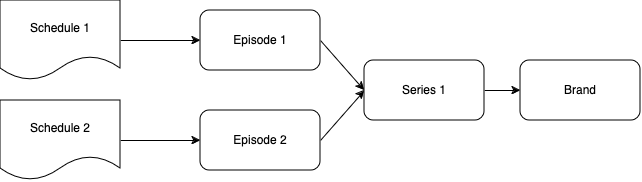
\includegraphics[width=8cm]{assets/catalogueTree.drawio.png}
    \caption{Example tree and associations between objects.}
    \label{fig:catalogueTree}
  \end{figure}

  Looking at the figure above outlines one possible scenario. If \emph{Episode 1} is removed from \emph{Schedule 1} then the episode object should be removed
  from redis and so should it's parent \emph{Series 1} as that also no longer has any schedule relations. However \emph{Brand} must stay as it still
  has \emph{Episode 2} and \emph{Series 2} that depend on it and relate it to \emph{Schedule 2}. Due to the potential to fan out like this, all data stored
  in the redis keyspace would have to be checked to see if there was any schedule still depending on the top level object (the brand). This takes a lot of
  memory and bandwidth to retrieve all this data. It was for that reason that it was decided, once a day a garbage collector should be ran to 
  tidy up anything no longer required.

  \begin{figure}[H]
    \centering
    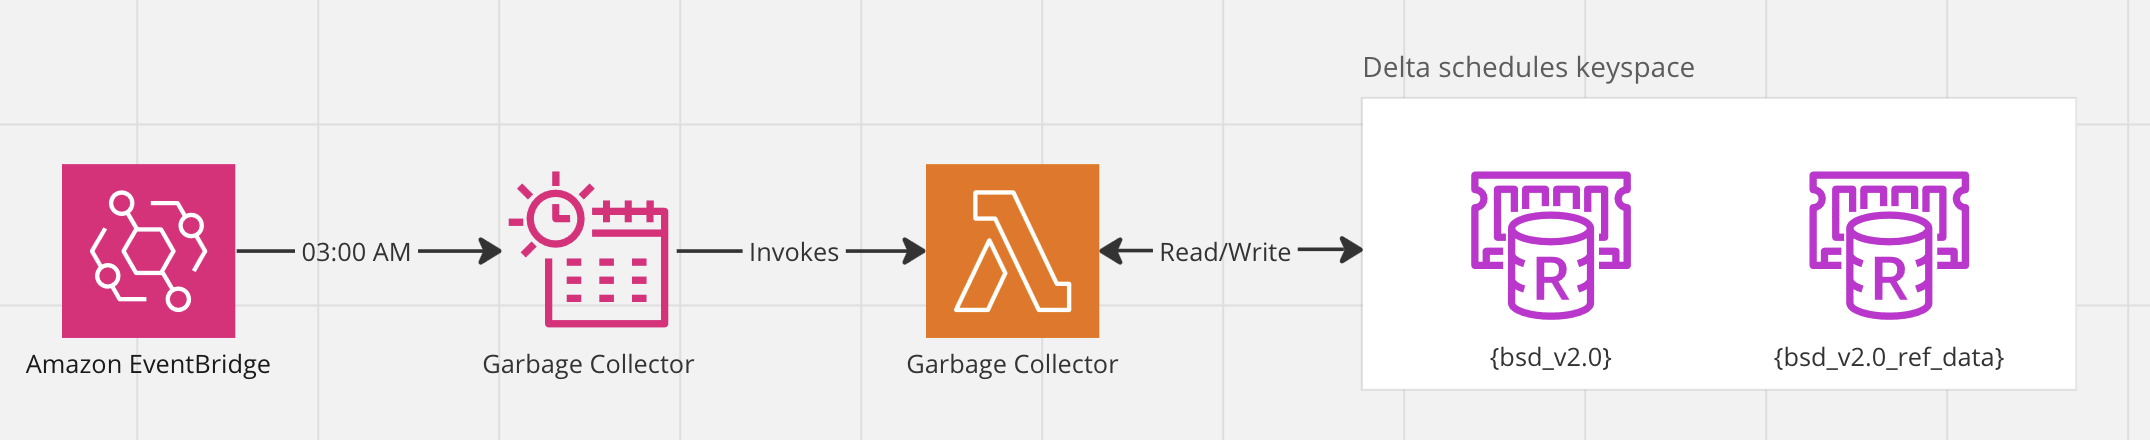
\includegraphics[width=8cm]{assets/architectures/garbageCollector.png}
    \caption{Garbage collector architecture.}
    \label{fig:garbageCollectorArchitecture}
  \end{figure}

  Above is the final architecture, a lambda is triggered by a scheduler once a day a 3AM to tidy up the leftover series and brands. In a later
  \hyperref[sec:garbageCollectorConsolidation]{\textbf{section}} the idea of moving all catalogue removals, including episodes, to the garbage 
  collector is explored.

  \newpage
  \subsubsection{End-to-end tests}
  In this section I want to discuss the larger tests that were created as part of the project. These include end-to-end (e2e) and comparison tests.
  As a team we follow the pattern of tests layed out in the test pyramid.

  \begin{figure}[H]
    \centering
    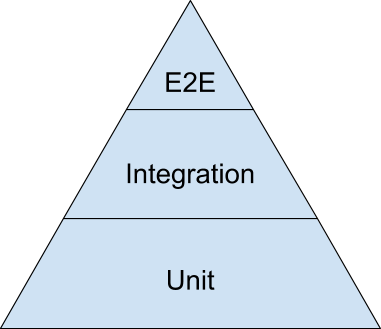
\includegraphics[width=6cm]{assets/testPyramid.png}
    \caption{Test pyramid (Wacker, 2015).}
    \label{fig:testPyramid}
  \end{figure}

  Unit tests and integration tests are written alongside the code, and can run on project build as they are cheap and quick to run (Spinellis, 2017).
  E2e tests sit at the top of this pyramid and should be used sparingly. This is not always the case, in other types of development, for example mobile,
  this pyramid can be turned upside down (Knott, 2015, cited in Contan, Dehelean and Miclea, 2018). This is probably due to mobile application being 
  primarily UI driven, which is the opposite for this project.

  In addition to this e2e and integration tests often get confused with one another. Integration tests \textit{'ensure synchronization between modules'}
  (Testim, 2021), and are more comparable to a unit test. Whereas a unit test is concerned on a single function/method an integration would test the calling of 
  methods by other methods and ensure integration between these two functions are working as expected. E2e tests are focused on actions/events that the 
  system must deal with as normal operation and could be described as automated manual testing (Testim, 2021).
  
  Due to their higher complexity, e2e tests are not without their potential problems. These include maintenance the written 
  tests, flakiness (are prone to randomly pass or fail without any discernable reason), time taken to run the tests and the cost of both the 
  execution of the tests and the time to write them (Yang and Leotta et al, 2023). 

  One of the larger problems we've faced in the passed is asynchronicity between tests (Leotta et al, 2023). For example if we upload a schedule at the 
  start of the pipeline and want to test it's structure at the end of the pipeline where partners would receive it, there's a lot that can interfere with 
  expected outputs. For the most part these bugs are when tidy up of a previous test is not carried out fully. If two test use the same identifier 
  for a schedule and then don't remove said schedule, this can result in tests not running how expected. It's for this reason during the development 
  of these new tests the code below was written to ensure that the schedule item about to be asserted on is not stored in the redis prior to the 
  test starting.

  \begin{lstlisting}[caption=Code to ensure schedule to asserted on is not present at the start of the test.]
    waitFor(`Ensure ${schedule} is not present before running test`, async () => {
      const bsd = await fetchFromRedis({
        command: 'isAbsent',
        keySpace: 'bsd_v2.0',
        sidDates: [schedule],
      })
      expect(bsd).toEqual([null])
    })
  \end{lstlisting} 

  Our current tests are written in \textit{scenarios} by our test team, a list of which can be seen in \hyperref[sec:AppendixG]{\textbf{Appendix G}}.
  Currently these cover all possible scenarios, however have a lot of overlap and repetitiveness. In an ideal world a test would cover an individual
  use case (Daly, 2022). These 14 scenarios could then be a part of these use case tests which would speed how quickly they run, thus lowering the cost.
  These use cases could be the following:

  \begin{itemize}
    \item Update a schedule
    \item Delete a schedule
    \item Update an episode
    \item Update an ancestor (series/brand)
    \item Tidy up orphaned items in redis (garbage collector)
  \end{itemize}

  This lowers the number of running test by 9 and removes a lot of time and duplication taken by setting up the scenarios. Due to time constraints and 
  prioritisation of other projects for the future, this refactor has not yet been undertaken but is in the backlog of things to do in the future. The 
  cost saved from changing this wouldn't be high, and doesn't justify the time it would take to refactor.

  For this project we stuck with the scenarios, some had already been done in previous work which meant we only had tests to write for the new 
  notification functionality. After discussion with the test team these tests include:

  \begin{enumerate}
    \item Hydration of episode stub to full episode object on episode update, as well as the episode parents and grandparents being transferred. This
    test would also make sure any schedules associated with the episodes titling was updated.
    \item Complex logic on schedule update, when a broadcasts episode changes in the schedule, if that episode has no remaining links to any other 
    schedules it should be removed from the schedule redis.
    \item Test whether correct supplementary data matches what is in the schedule. For partner requests we also send episode/series/brand data, 
    this data should be relevant to the broadcasts contained within the schedule.
  \end{enumerate}

  There were originally more test scenarios to be done as part of this project. However after discussing with both developers and testers it was decided 
  that these were either already being tested by unit tests or other parts of the testing library, or were unnecessary. This work was removed from 
  the board which can be seen in the burn-up charts in the \hyperref[sec:burnup]{\textbf{Outputs}} section.

  Finally we created comparison tests, to compare the old static output and new delta/notification output. These tests could be compared to extract, 
  transform, load (ETL) testing (Talend Inc, 2024). These tests will give us the confidence to switch our partners over to the new system. We decided
  upon a 1 week time frame where these comparisons tests must pass continuously before we are happy to make the switch. On failure the logs from the test
  will help us debug any current and future issues with the system.

  \newpage